\documentclass{article}

\usepackage{geometry}
\usepackage{makecell}
\usepackage{array}
\usepackage{multicol}
\usepackage{setspace}
\usepackage{changepage}
\usepackage{amsmath}
\usepackage{booktabs}
\usepackage{amssymb}
\usepackage[explicit]{titlesec}
\usepackage{hyperref}
\usepackage{graphicx}
\usepackage{cprotect}
\usepackage{float}
\newcolumntype{?}{!{\vrule width 1pt}}
\newcommand{\paragraphlb}[1]{\paragraph{#1}\mbox{}\\}
\newcommand{\subparagraphlb}[1]{\subparagraph{#1}\mbox{}\\}
\renewcommand{\contentsname}{Inhaltsverzeichnis:}
\renewcommand\theadalign{tl}
\makeatletter
\newcommand{\Spvek}[2][r]{%
  \gdef\@VORNE{1}
  \left(\hskip-\arraycolsep%
    \begin{array}{#1}\vekSp@lten{#2}\end{array}%
  \hskip-\arraycolsep\right)}

\def\vekSp@lten#1{\xvekSp@lten#1;vekL@stLine;}
\def\vekL@stLine{vekL@stLine}
\def\xvekSp@lten#1;{\def\temp{#1}%
  \ifx\temp\vekL@stLine
  \else
    \ifnum\@VORNE=1\gdef\@VORNE{0}
    \else\@arraycr\fi%
    #1%
    \expandafter\xvekSp@lten
  \fi}
\makeatother

\newcommand{\N}{\mathbb{N}}
\newcommand{\Z}{\mathbb{Z}}
\newcommand{\Q}{\mathbb{Q}}
\newcommand{\R}{\mathbb{R}}
\newcommand{\M}{\mathbb{M}}
\setstretch{1.10}
\setlength{\parindent}{0pt}
\setcounter{tocdepth}{5}

\titleformat{\section}
  {\normalfont\Large\bfseries}{\thesection}{1em}{\hyperlink{sec-\thesection}{#1}
\addtocontents{toc}{\protect\hypertarget{sec-\thesection}{}}}
\titleformat{name=\section,numberless}
  {\normalfont\Large\bfseries}{}{0pt}{#1}

\titleformat{\subsection}
  {\normalfont\large\bfseries}{\thesubsection}{1em}{\hyperlink{subsec-\thesubsection}{#1}
\addtocontents{toc}{\protect\hypertarget{subsec-\thesubsection}{}}}
\titleformat{name=\subsection,numberless}
  {\normalfont\large\bfseries}{\thesubsection}{0pt}{#1}

\hypersetup{
    colorlinks,
    citecolor=black,
    filecolor=black,
    linkcolor=black,
    urlcolor=black
}

\geometry{top=12mm, left=1cm, right=2cm}
\title{\vspace{-1cm}Mathematik für Informatik 2}
\author{Andreas Hofer}

\begin{document}
	\maketitle
	\tableofcontents
	\section{Kombinatorik}
	Die Kombinatorik ist die Vorstufe der Wahrscheinlichkeitstheorie und beantwortet allgemeine Fragen des Abzählens. Zum Beispiel, wenn man wissen will wie viele Möglichkeiten es gibt Objekte anzuordnen und auszuwählen. Zum Beispiel wenn man eine bestimmte Menge an möglichen Ausgängen ermitteln will (Die Menge an verschiedenen Würfelpositionen). Dabei unterscheidet man zwischen den günstigen und den möglichen Fällen. Günstige Fälle sind jene die man erhalten will, während die möglichen Fälle die Summe aller Fälle ist. Ein spezieller Fall der Wahrscheinlichkeit ist das Laplace-Experiment, in welchem jeder Ausgang die gleiche Wahrscheinlichkeit hat. (Zum Beispiel ein Würfel, welcher stets eine Chance von 1/6 hat).
	\subsection{Abzählverfahren}
	Bei den Abzählverfahren der Kombinatorik existieren drei fundamentale Regeln:
	\subsubsection{Summenregel}
	Bei zwei endlichen disjunkten (Mengen ohne gemeinsame Elemente) Mengen gilt, dass die Vereinigung der Mengen die selbe Mächtigkeit hat als die Summe dieser zwei Mengen: $|A \cup B|=|A|+|B|$. Die Union der Mengen hat somit die gleiche Menge an Elementen, als die Summe der beiden Mengen. Das ist relevant in Fällen, in denen Eigenschaften eines Objektes sich einander ausschließen. Zum Beispiel kann man ein Auto nur entweder als Kleinwagen oder als Mittelklassewagen klassifizieren, jedoch nie beides.
	\paragraphlb{Verallgemeinerung}
	Für diese Regel existiert auch einen Verallgemeinerung, bei der mehr als zwei Mengen verwendet werden kann. Eine Regel dabei ist, dass der Schnitt jeder Menge die leere Menge ergibt.
	\subsubsection{Produktregel}
	Anders als bei der Summenregel müssen bei der Produktregel die Mengen nicht disjunkt sein. Hierbei wird das kartesische Produkt der Mengen gebildet: $|AxB|=|A|\cdot|B|$. Ein Beispiel zur Anwendung ist die Routenplanung. Angenommen es gibt drei Routen von Wien nach Graz und 4 Routen von Wien nahc Marburg, kann man diese kombinieren, da man eine beliebige Route von Wien nach Graz und eine beliebige Route von Graz nach Marburg verwenden kann. So gibt es ingsesamt 12 verschiedene Möglichkeiten von Wien nach Marburg zu kommen, da man jede der ersten Route mit jeder der zweiten Route kombinieren kann.
	\paragraphlb{Verallgemeinerung}
	Auch bei der Produktregel existiert eine Verallgemeinerung mit beliebig vielen Schritten. Dabei wird wieder die Mächtigkeit jeder Teilmenge mit jeder anderen Teilmenge multipliziert. Ein Beispiel dafür ist die Menge der Möglichkeiten bei einer Binärzahl. So hat man 8 Bits zur Verfügung und jedes Bit kann zwei Mögliche Zustände (1 und 0) besitzen, wodurch man diese zwei Möglichkeiten acht Mal miteinander multipliziert um zum Ergebnis zu kommen: $2^8=256$
	\subsubsection{Kombination}
	Man kann die Summen- und Produktregel auch miteinander kombinieren. Dabei muss man zuerst die Möglichen Ausgänge kombinieren und dann jeweil die Kombinationen multiplizieren: Angenommen man hat ein Passwort das aus Ziffern und Buchstaben bestehen kann, kombiniert man die 10 Ziffern und 26 Buchstaben zu je 36 Möglichkeiten, welche danach normal miteinander kombiniert werden. \\
	Wenn man eine Einschränkung hat, dass mindestens eine Ziffer vorkommen muss, hat man zwei Möglichkeiten diese zu berechnen:
	\begin{enumerate}
		\item{Man berechnet die Menge aller Möglichkeiten mit Ziffern und Buchstaben und zieht davon alle Möglichkeiten welche nur Buchstaben enthalten ab}
		\begin{itemize}
			\item{$P_6 - ($Menge an Passwörtern ohne Ziffern$) = P_6 - 26^6 = 36^6 - 26^6 = 1.867.866.560$}
		\end{itemize}
		\item{Man nimmt jede Ziffer diskret wahr und berechnet anhand dessen dann die Menge an Möglichkeiten pro Ziffer}
		\begin{itemize}
			\item{10*36*36*36*36*36 + 26*10*36*36*36*36 + 26*26*10*36*36*36 + 26*26*26*10*36*36 + 26*26*26*26*10*36 + 26*26*26*26*26*10 = 1.867.866.560}
		\end{itemize}
	\end{enumerate}
	\subsubsection{Exklusion/Inklusion}
	Zur Anwendung der Summenregel bei nicht-disjunkten Mengen (Wenn also Werte in beiden Mengen vorkommen) gibt es die Verallgemeinerung dessen. Um einen Wert nicht zwei Mal zu zählen muss man diese so zuerst normal vereinen, danach aber die Schnittmenge der Mengen davon wieder abzuziehen: $|A\cup B| = |A|+|B|-|A\cap B|$ \\
	Wenn zum Beispiel in einer Stadt 1.000.000 Menschen leben, welche jeweils Deutsch und/oder Französisch sprechen und 90\% zumindest Deutsch und 20\% zumindest Französisch, wie viele sprechen dann beide Sprachen? Um das Ergebnis zu erhalten, muss man dabei die Schnittmenge der beiden Mengen erhalten, da man ja die Anzahl der Werte die in beiden Mengen enthalten sind wissen will: $|D\cap F| = |D| + |F| - |D\cup F| =$ \\
	Ein weiteres Beispiel ist die Frage, wie viele 8-stellige Binärzahlen es gibt, die mit 0 beginnen oder mit 11 enden. Da Binärzahlen nur zwei Möglichkeiten haben, kann man die festen Stellen ignorieren (Da es nur mehr eine Möglichkeit gibt). So erhält man $2^7$ Zahlen, die mit 0 beginnen und $2^6$ Zahlen die mit 11 enden. Diese Zahlen inkludieren sich jedoch jeweils selbst, wodurch man alle Zahlen die beide Eigenschaften aufweisen abziehen muss. Da Zahlen von der Form 0XXXXX11 doppelt gezählt werden und es $2^5$ davon gibt, muss man diese wiederum von den Möglichkeiten abziehen. So erhält man die Formel $2^7+2^6-2^5=160$ 
	\subsection{Permutation und Kombination}
	Bei der Permutation und Kombination wird unterschieden, ob die Reihenfolge der Element eine Rolle spielt oder nicht. Bei beiden Varianten besteht die Möglichkeit das gewählte Element wieder zurückzulegen, wodurch es bei der nächsten Auswahl wieder zur Verfügung steht. Also kann es jeweils um eine Permutation oder Kombination mit oder ohne Zurücklegen handeln.
	\subsubsection{Permutation}
	Bei der Permutation spielt die Reihenfolge der Elemente aus der Menge eine Rolle. Man spricht auch von geordneter Auswahl, Variation oder k-Permutation. 
	\paragraphlb{Ohne Zurücklegen}
	Bei der Permutation ohne Zurücklegen ist die Reihenfolge relevant, wobei nach jeder Wahl die Menge der möglichen Werte verringert wird. Bei einer 3-Permutation werden dabei alle Kombinationen an Werten, welche nach drei Runden gewählt werden können angegeben. \\
	Die Anzahl der k-Permutationen aus einer Menge mit n Elementen wird als P(n, k) bezeichnet und ist gegeben durch: $P(n, k)=n*(n-1)*(n-2)*...*(n-k+1)=\frac{n!}{(n-k)!}$ \\
	Es existiert auch ein Spezialfall, wenn die Menge der Permutationen und die Anzahl der Element die gleiche ist. In diesem Fall kann man es durch $n!$ berechnen. Diese lässt sich aus der oberen Formel herleiten, da unter der Klammer (n-n)! gleich 1 ist und somit wegfällt. \\
	Ein Beispiel für eine Permutation ist, die Frage über die Anzahl der Möglichkeiten 5 Bilder nebeneinander an der Wand aufzuhängen. Da man ein Bild das man bereits aufgehängt hat, nicht noch ein Mal aufhängen kann, verringern sich die Möglichkeiten mit jedem Bild. Da jedoch auch jedes Bild aufgehängt wird, ist die Menge der Permutationen gleich der Anzahl der Elemente, wodurch es als n! angegeben werden kann: $5!=120$
	\paragraphlb{Mit Zurücklegen}
	Wenn ein Wert zurückgelegt wird, steht er für weitere Ziehungen wieder zur Verfügung und kann dadurch auch mehrmals vorkommen. Im Falle der Permutation ist die Formel $n^k$ und wurde auch bereits verwendet, zum Beispiel bei den Pinexperimenten.
	\subsubsection{Kombination}
	Bei der Kombination spielt die Reihenfolge keine Rolle und wird auch als Ungeordnete Auswahl bezeichnet. Eine Kombination entspricht genau einer Teilmenge. 
	\paragraphlb{Ohne Zurücklegen}
	Die Anzahl der möglichen Kombinationen wird als C(n, k) geschrieben und kann mit $\frac{P(n, k)}{k!} oder \frac{n!}{k!(n-k)!}$ berechnet werden. \\
	Kombinationen sind relevant wenn man ein Team uas einer bestimmten Menge an Personen wählen will. Da es keinen Unterschied macht ob man zuerst Person 1 oder Person 2 wählt. Wenn man also eine Gruppe aus 4 Personen hat und ein zweiköpfiges Team bilden will, berechnet man das mit $\frac{P(4,2)}{2!}=\frac{4!}{2!(4-2)!}=\frac{4!}{2!2!}=\frac{24}{4}=6$
	\paragraphlb{Mit Zurücklegen}
	Die Kombination mit Zurücklegen basiert auf dem gleichen Prinzip, kombiniert jedoch alle möglichen Kombinationen aus Werten. Die Formel ist: $\binom{n+k-1}{k}$. Da man die Werte stets wieder zurücklegt, wird die Formel behandelt, als ob sie die Elemente plus alle zurückgelegten Elemente enthält.
	\subparagraphlb{Beispiel}
	Ein Beispiel ist eine Stichprobe mit 10 PCs, wobei 3 Geräte fehlerhaft sind. Wenn man einer Lieferung eine Stichprobe von 5 Geräten entnimmt, wie viele Stichproben enthalten dann genau zwei defekte Geräte? \\
	Diese Aufgabe muss in zwei Schritten gelöst werden. Zuerst muss die Menge der Stichproben mit genau zwei defekten Geräten ermittelt werden: $C(3,2)=\binom{3}{2}=3$. \\
	Danach muss man die Menge an Stichproben mit genau drei funktionierenden Geräten aus den 7 funktionierenden ermitteln: $C(7,3)=\binom{7}{3}=35$ \\
	Diese msus man nun mit der Produktregel kombinieren: C(3,2)*C(7,3)=3*35=105. \\
	Wenn man stattdessen wissen will, wie viele Stichproben mit mindestens einem defekten Gerät existieren
	\subsubsection{Binomialkoeffizient}
	Eine alternative Schreibweise für die Kombination ohne Zurücklegen, ist der Binomialkoeffizient. Diese wird als $\binom{n}{k}$ geschrieben und beschreibt die gleiche Formel.
	\paragraphlb{Lehrsatz}
	Der binomische Lehrsatz besagt, dass $(x+y)^n$ gleich $\sum_{k=0}^{n}\binom{n}{k}x^{n-k}y^k$. Mithilfe diese Lehrsatzes kann man für ein beliebiges n die binomische Formel herleiten.
	\paragraphlb{Mit Zurücklegen}
	\section{Vektoren}
	Vektoren beschreiben die Verwaltung von n-Tupeln, welche multidimensionale Systeme darstellen. Vektoren werden umfangreich in Gleichungssystemen und Kryptographie verwendet. Die Eigenschaft eines Vektors ist, dass sie nicht nur einen Betrag (den Wert) sondern auch eine Richtung hat. Ein Vektor erweitert deshalb einen Skalar (wie die Zahl 5) um eine weitere Eigenschaft. Vektoren sind stets Element eines Vektorraums, wie $R_2$, welche nur im zweidimensionalen Raum existieren (Zum Beispiel x und y). \\
	Ein Vektor kann theoretisch unendlich viele Werte besitzen und wird beschrieben als $(a_1,a_2,a_3,...,a_n)\in \R^n$ wobei $a_1$ bis $a_n$ die Koordinaten des Vektors und $\R^n$ den Vektorraum beschreiben. \\
	Ein Vektor wird üblicherweise mit einem Pfeil über der Bezeichnung geschrieben: [TODO PFEIL a] und als Spaltenvektor oder Zeilenvektor $a_1,a_2,a_3,...,a_n)$. \\
	\subsection{Darstellung}
	Vektoren können auf verschiedene Weisen dargestellt werden:
	\subsubsection{Ortsvektor}
	Ein Ortsvektor ist in ein Vektor in $\R^2$ oder $\R^3$ mittels Pfeil. Für höhere Dimensionen ist es nicht wirklich möglich. Der Ausgangspunkt für einen Ortsvektor ist dabei der Ursprung (0,0) welcher zu den Koordinaten führt: $\textbf{a}=\vec{a}$=[TODO OP MIT PFEIL]=Q(5|6). \\
	Ein Vektor muss jedoch nicht vom Ursprung beginnen. In diesem Fall wird der Ausgangspunkt nicht mit O sondern mit einem anderen Vektor bezeichnet: $\textbf{b}=\vec{b}$=[TODO PQ] \\
	Wenn man einen Vektor als Orientierung zwischen zwei Punkten verwendet, muss man \textbf{Spitze minus Schaft} rechnen: [AB]=$\begin{pmatrix}x_B-x_A \\ y_B-y_A \end{pmatrix}$ \texttt{ -> } [TODO Vector SLIDE 10]
	\subsection{Rechenoperationen}
	\subsubsection{Addition/Subtraktion}
	Vektoren kann man gleich wie Skalare addieren und subtrahieren. Dabei werden diese elementweise verbunden, müssen jedoch stets aus dem selben Vektorraum sein: $\textbf{a + b}=\vec{a}+\vec{b}=\begin{pmatrix} a_1+b_1 \\ a_2+b_2 \\ a_3+b_3 \\ ... \\ a_n+b_n\end{pmatrix}$ \\
	Hierbei werden die Vektoren direkt miteinander kombiniert und es entsteht ein neuer Vektor im gleichen Raum.
	\begin{figure}[H]
	\centering
	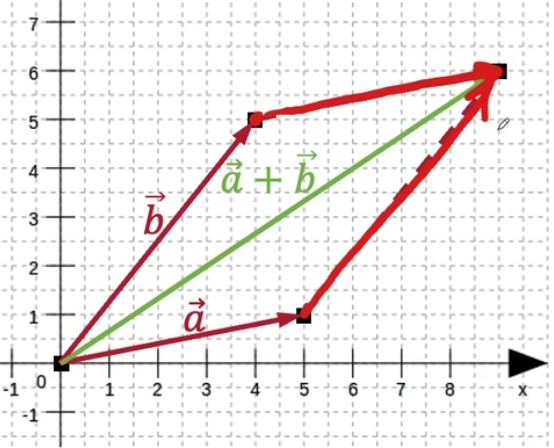
\includegraphics[scale=0.5]{Bilder/vector_add.png}
	\caption{Vektoraddition}
	\end{figure}
	\subsubsection{Multiplikation}
	\paragraphlb{Mit Skalar}
	Man kann einen Vektor auch multiplizieren, dabei diesen jedoch auch mit einem Skalar verbinden wobei jedes Element des Vektors mit diesem Skalar multipliziert wird: $\textbf{a}*k=\vec{a}*k=\begin{pmatrix} a_1*k \\ a_2*k \\ a_3*k \\ ... \\ a_n*k\end{pmatrix}$ \\
	\paragraphlb{Skalarprodukt}
	Wenn man zwei Vektoren miteinander multipliziert erhält man am Ende einen Skalar. Dabei wird jedes Element eines Vektors mit dessen Paar multipliziert, welche danach addiert werden. $\textbf{a*b}=\vec{a}*\vec{b}=a_1*b_1+a_2+b_2+...+a_n*b_n$. Das Skalarprodukt wird als $\vec{a}\cdot\vec{b}$ geschrieben
	\subsubsection{Gleichheit}
	Die Gleichheit von Vektoren ist gegeben wenn jedes Element eines Vektors gleich ist wie das passende Element des anderen Vektors: \textbf{a=b}$=a_1=a_2, a_2=a_3$
	\subsection{Beispiele}
	Gegeben: $\vec{a}=(x-1,2y,x+z), \vec{b}=(0,4,-1)$ \\
	Gesucht: Die reellen Zahlen x, y und z sodass $\vec{a}=\vec{b}$ \\
	$\vec{a}=\vec{b}=\begin{pmatrix} x-1 \\ 2y  \\ x+z \end{pmatrix}=\begin{pmatrix} 0 \\ 4 \\ -1  \end{pmatrix}$
	\subsubsection{Skalarprodukt}
	Gegeben: $\vec{a}=(1,3,5), \vec{b}=(2,0,4)$ \\
	Gesucht: $\vec{a}\cdot\vec{b}$ \\
	$\vec{a}\cdot\vec{b}=\begin{pmatrix} 1 \\ 3 \\ 5 \end{pmatrix}\cdot \begin{pmatrix} 2 \\ 0 \\ 4 \end{pmatrix}=1*2+3*0+5*4=2+0+20=22$
	\subsection{Vektorraum}
	Der Vektorraum ist wie bereits erwähnt die Gesamtheit aller Vektoren die die gleichen Eigenschaften besitzen (Die gleiche Menge an Elementen). In einem Raum gelten folgende Regeln:
	\subsubsection{Addition}
	\begin{itemize}
		\item{Kommutativität}
		\begin{itemize}
			\item{$\vec{a}+\vec{b}=\vec{b}+\vec{a}$}
		\end{itemize}
		\item{Assoziativität}
		\begin{itemize}
			\item{$(\vec{a}+\vec{b})+\vec{c}?\vec{a}+(\vec{b}+\vec{c})$}
		\end{itemize}
		\item{Neutrales Element}
		\item{Inverses Element}
	\end{itemize}
	\subsubsection{Multiplikation}
	\begin{itemize}
		\item{Assoziativität}
		\begin{itemize}
			\item{$k(h \vec{a})=(kh)\vec{a}$}
		\end{itemize}
		\item{Neutrales Element}
		\begin{itemize}
			\item{$1 \vec{a}=\vec{a}$}
		\end{itemize}
		\item{Distributivität}
		[TODO REGELN]
	\end{itemize}
	\subsection{Vektorlänge}
	Vektoren mit mehr als drei Komponenten lassen sich grafisch nur bedingt veranschaulichen, haben jedoch auch außerhalb von grafischer Darstellung einen Nutzen. Die Länge eines Vektors ist der Betrag dessen Komponenten. Also kann man mit dem Satz des Pythagoras die Länge eines Vektors bestimmen (Da die Länge eines Vektors die Hypothenuse eines gespannten Dreiecks ist.) $||\vec{a}||=\sqrt{a^2+b^2}$. \\
	Diese Regel ist auch für Vektoren mit mehr als 2 oder 3 Elementen anwendbar: $||\vec{a}||=\sqrt{\sum_{j=1}^{n}a_j^2=\sqrt{a_1^2+a_2^2+a_3^2+...+a_n^2}}$ \\
	Der Betrag ist immer eine nichtnegative reelle Zahl, selbst wenn der Vektor selbst negativ ist. Gleichzeitig ist der Betrag nur 0, wenn alle Elemente des Vektors 0 sind. \\
	Man kann dies auch verwenden um den Abstand zweier Punkte berechnen: $||\overrightarrow{AB}||=\sqrt{(B_1-A_1)^2+(B_2-A_2)^2+...+(B_N-A_N)^2}$ \\
	Im Falle des Abstands ist die Reihenfolge der Vektoren jedoch unwichtig. Ob man also A von B abzieht oder B von A führt zum gleichen Ergebnis.
	\subsection{Einheitsvektor}
	Ein Einheitsvektor ist ein Vektor mit der Länge 1. Ein Einheitsvektor eines beliebigen Vektors hat die selbe Richtung als dieser Vektor mit der Länge von 1. Diesen berechnet man indem man ihn durch die Inverse der Länge des Vektors dividiert: ${\frac{1}{||\vec{a}||}\vec{a}}$. Einheitsvektoren werden häufig bei Matrizenrechnungen verwendet
	\subsection{Vektornormen}
	Eine Vektornorm ist ein Raum in dem eine Norm definiert ist. Die Norm ist die Verallgemeinerung des geometrischen Begriffs der Länge: $||\cdot||:V\rightarrow [0, \infty)]$. Sie ordnet also jedem Element eines Vektorraums eine nichtnegative reelle Zahl zu. \\
	Normen müssen einige Bedingungen erfüllen:
	\begin{itemize}
		\item{Positivität - Jede Norm ist eine Positive Zahl (Ausnahme ist der Nullvektor)}
		\item{Definitheit - }
		\item{Absolute Homogenität - }
		\item{Subadditivität - Die Norm zweier addierter Vektoren ist definitiv kleiner (oder maximal gleich) als die Summe der Normen der separaten Vektoren}
	\end{itemize}
	\subsubsection{P-Norm}

	\paragraphlb{Betragssummennorm}
	Die Betragssummennorm, auch 1-Norm genannt ist eine p-Norm mit dem Wert 1: $||x||_1:=\sum_{i=1}^{n}|xi|$ \\
	Die Betragssummennorm eines Vektors ist die Summe des Betrags aller Komponenten eines Vektors. Das entspricht den Längen der Achsen des Vektors.
	\paragraphlb{Euklidische Norm}
	Die Euklidische Norm, auch 2-Norm genannt ist die gleiche Formel mit dem Wert 2: $||x||_2:=\sqrt{\sum_{i=1}^{n}}$. Das entspricht genau der Länge des Vektors selbst.
	\paragraphlb{Teschebyschow Norm}
	Hierbei wird das Maximum der Komponenten genommen. Dabei wird der Betrag jedes Elements eines Vektors herangezogen und das Maximum genommen. Wenn ein Vektor also die Werte 1, 2 und -3 enthält, wäre das Maximum 3, da der Betrag von -3 der höchste Wert ist. Das entspricht der einzelnen längsten Länge des Vektors.
	\subsection{Lineare Unabhängigkeit}
	Vektoren sind jeweils entweder linear abhängig oder unabhängig voneinander. Ein Vektor ist linear abhängig von einem anderen Vektor, wenn diese parallel zueinander stehen. Vektoren sind genau dann linear unabhängig wenn man in der Vektorgleichung $k_1 \vec{a_1}+k_2 \vec{a_2}+...+k_m \vec{a_m}=\vec{0}$ erhält, wobei jedes k gleich 0 ist und \textit{das die einzige Möglichkeit ist} um das Ergebnis zu erhalten. Falls das nicht möglich ist, sind zwei Vektoren linear abhängig. Auch wenn sich nur einer der Vektoren als Linearkombination schreiben lässt, sind diese linear abhängig. Per Definition ist auch ein Nullvektor linear abhängig. Das bedeutet, dass Vektoren linear unabhängig sind, wenn es keine k gibt, die nicht alle 0 sind, für welche man den Nullvektor bilden kann.
	\subsubsection{Komplanar}
	Drei Vektoren sind abhängig, wenn sie in einer Ebene durch Verlängerung oder Verkürzung eine Ebene bilden. Im zweidimensionalen Raum sind ab einer gewissen Länge alle Vektoren komplanar. In einem dreidimensionalen Raum können Vektoren jedoch unabhängig sein, wenn sie in einer anderen Dimension stehen. \\
	Man kann Vektoren kombinieren, indem Vektoren mit beliebigen Skalaren verbunden werden. Dabei wird jeder Vektor mit einem Skalar multipliziert und danach aufaddiert. Das Resultat ist ein neuer Vektor. \\
	Um eine Linearkombination zu ermitteln, muss man für zwei Vektoren ein lineares Gleichungssystem bilden. $\sum_{j=1}^{m}k_j \vec{a_j})k_1*\vec{a_1}+k_2+...+k_m*\vec{a_m}$ \\
	In diesem Fall existiert eine eindeutige Lösung. Das funktioniert, da diese beiden Vektoren linear unabhängig sind. Man kann für jeden beliebigen Vektor eine Lösung finden, falls die Vektoren linear unabhängig voneinander sind.
	\subsection{Vektorbasis}
	Einheitsvektoren entlang drei verschiedener Achsen sind jeweils linear unabhängig: $\vec{e_1}=(1,0,0),\vec{e_2}=(0,1,0),\vec{e_3}=(0,0,3)\in\R^3$. Ein weiterer Vektor in diesem Raum würde die lineare Unabhängigkeit jedoch zerstören. Die drei Einheitsvektoren $e_1,e_2,e_3$ bilden die Standardbasis. \\
	Mit einer Basis kann man jeden beliebigen Vektor aus dem selben Vektorraum darstellen: $\vec{a}=\sum_{j=1}^{n}k_j \vec{e_j}$. So kann man einen Vektor stets als Linearkombination von Standardvektoren darstellen. \\
	Eine Basis besteht stets aus einer Familie aus Vektoren die wiederum aus n linear unabhängigen Vektoren besteht. Dabei muss es stets alle Dimensionen eines Raumes ausgeschöpft werden (Also 3 Vektoren im Raum $\R^3$). Innerhalb dieses Raums lässt sich jeder Vektor als Kombination dieser Vektoren darstellen. \\
	\paragraphlb{Beispiel}
	Gegeben sind drei linear unabhängige Vektoren: $\vec{a_1}=(2,0,1),\vec{a_2}=(1,2,0),\vec{a_3}=(0,0,2)$ \\
	Gesucht werden die Koordinaten (1,-10,4) bezüglich der Basis: $k_1 \vec{a_1}+k_1 \vec{a_2}+k_3 \vec{a_3}=\begin{pmatrix} 1 \\ -10 \\ 4 \end{pmatrix}$ \\
	$k_1 \begin{pmatrix} 2 \\ 0 \\ 1 \end{pmatrix}+k_2 \begin{pmatrix} 1 \\ 2 \\ 0 \end{pmatrix}$ [TOOD SLIDE 68]
	\subsection{Dimension}
	Die Dimension ist die maximale Anzahl linear unabhängiger Vektoren in einem Raum und wird geschrieben als dim(V) und $dim(\R^n)=n$. Die Definition beschreibt die maximale Anzahl, da auch bei weniger Vektoren eine lineare abhängigkeit erreicht werden kann.
	\subsection{Geraden und Ebenen}
	Die Geradengleichung war stets in der parameterfreien Form. Die Parameterform beschreibt stattdessen Vektoren: $g:\vec{x}=\vec{p}+h \vec{r}$
	\begin{itemize}
		\item{$\vec{x}$ - Beschreibt den Ortsvektor $\overrightarrow{0X}$ eines Punkts X auf der Geraden}
		\item{$\vec{p}$ - Beschreibt einen Ortsvektor $\overrightarrow{0P}$ eines Punkts P}
		\item{$\vec{r}$ - Beschreibt den Richtungsvektor der Geraden}
		\item{h - }
	\end{itemize}
	\paragraphlb{Beispiel}
	Gegeben ist P(2|-1),$\vec{r}$=(1,5) wobei die Geradengleichung gesucht wird. \\
	Man kann einfach in die Geradengleichung einsetzen: $g:\vec{x}=\vec{p}+h \vec{r}$\texttt{ -> }$\vec{x}=\begin{pmatrix} 2 \\ -1 \end{pmatrix}+h \begin{pmatrix} 1 \\ 5 \end{pmatrix}$ \\
	Diese Parametergleichung kann man in die Normalform überbringen indem man diese mit einem linearen Gleichungssystem löst: \\
	\begin{itemize}
		\item[I]{$2+1h$ \texttt{ -> } Multipliziert mit 5}
		\item[II]{$-1+5h$}
		\item[5*II]{$5x=10+5h$}
		\item[5*II-I]{$5x-y=10+5h-(-1+5h)=11$ \texttt{ -> }$y=5x-11$}
	\end{itemize}
	\subsubsection{Ebenengleichung}
	Eine Ebene in einem Raum wird definiert durch den Punkt P mit dem Ortsvektor/Stützvektor $\vec{p}$ und den Richtungsvektoren $\vec{r}$ und $\vec{s}$. Dabei dürfen die Vektoren $\vec{r}$ und $\vec{s}$ nicht parallel sein. \\
	Eine Ebene kann auch in Parameterform stehen: $\epsilon:\vec{x}=\vec{p}+h \vec{r}+i \vec{s}$
	Es existiert auch wiederum eine Parameterfreie Form: [TODO] \\
	\section{Matrizen}
	Matrizen kann man als mehrdimensionale Vektoren verstehen. Es wird geschrieben als rechteckiges Zahlenschema. Man spricht in der Regel von einem m$\times$ n Schema, welches aus m Zeilen und n Spalten besteht. Eine Matrix wird geschrieben mit gerundeten Klammern als mehrdimensionaler Vektor. \\
	Vektoren sind spezielle Matrizen. Aus diesem grund sind Spalten- und Zeilenvektoren auch Matrizen. Ein Spaltenvektor ist eine Matrix mit einer Zeile und m Spalten, wobei ein Zeilenvektor eine Spalte und n Zeilen besitzt. \\
	Auch ein Skalar ist eine spezielle Matrix, nämlich mit einer Spalte und einer Zeile.
	\subsection{Nullmatrix}
	Ein Nullmatrix ist eine spezielle Matrix welche nur mit 0 gefüllt ist.
	\subsection{Quadratische Matrix}
	Eine Quadratische Matrix ist eine Matrix bei welcher die Anzahl der Spalten und Zeilen die selbe ist.
	\subsection{Dreiecksmatrix}
	Eine Dreiecksmatrix ist eine quadratische Matrix, welche nur Werte in einer Hälfte der Matrix enthält. Dabei wird zwischen der oberen und der unteren Dreiecksmatrix unterschieden, wobei nur die Hälfte oberhalb oder unterhalb der Hauptachse Werte enthält und alle anderen 0 sind (Die Werte können jedoch auch 0 sein).
	\subsection{Diagonalmatrix}
	Die Diagonalmatrix ist eine weitere spezielle Quadratische Matrix, welche außerhalb der Hauptdiagonale nur 0 besitzt.
	\subsection{Einheitsmatrix}
	Die Einheitsmatrix ist eine Diagonalmatrix, welche auf der Hauptdiagonale nur 1 besitzt. Es wird oft mit I benannt, nach der englischen Bezeichnung von "Identity Matrix". Die Einheitsmatrix hat den gleichen Effekt wie die Zahl 1 bei normalen Berechnungen, da sie immer die selbe Matrix als Ergebnis hat mit der sie multipliziert wurde.
	\subsection{Transponierte Matrix}
	Eine transponierte Matrix ist eine Matrix, bei welcher Zeilen und Spalten vertauscht wurden. Sie wird geschrieben als hochgestelltes T: $(a_{ij})^T=(a_{ji})$
	\subsection{Symmetrische Matrix}
	Eine Matrix ist eine quadratische Matrix, bei welcher die Werte ober und unter der Hauptachse gleich sind. Die formale Definition ist, dass eine Matrix symmetrisch ist, wenn die transponierte Matrix diese nicht verändert: $A=A^T$
	\subsection{Rechenregeln}
	\subsubsection{Gleichheit}
	Zwei Matrizen sind gleich $A=B$, wenn sie die gleiche Menge an Dimensionen besitzt und alle Werte an den gleichen Stellen die gleichen Werte besitzen.
	\subsubsection{Addition}
	Gleich wie bei Vektoren müssen Matrizen vom selben Typ sein damit sie addiert oder subtrahiert werden können: $A+B, A-B$ \\
	Matrizen können auch mit Skalaren multipliziert werden
	\subsubsection{Multiplikation}
	Die Multiplikation zweier Matrizen ist eine etwas komplexere Angelegenheit. Bei der Multiplikation müssen die beiden Matrizen im Format $m\times p$ A und $p\times n$ B. Dabei muss die Spaltenanzahl der Matrix A gleich der Zeilenanzahl der Matrix B sein. \\
	Dabei entsteht eine neue Matrix mit der Spaltenanzahl der Ersten und Zeilenanzahl der Zweiten: $(\textcolor{red}{m},\textcolor{green}{p})\cdot(\textcolor{green}{p},\textcolor{blue}{n})=(\textcolor{red}{m},\textcolor{blue}{n})$ \\
	Also wird aus der Multiplikation einer Matrix mit m Zeilen und p Spalten A und p Zeilen und n Spalten B zu einer neuen Matrix mit m Zeilen und n Spalten. \\
	Die multiplikation geschieht indem von jeder Zeile und Spalte das Skalarprodukt gebildet wird. Bei der Multiplikation gilt das Kommutativgesetz \textbf{nicht}. Also ist AB nicht gleich BA.
	\subsection{Inverse Matrix}
	Wenn man eine quadratische Matrix A und dessen inverse Matrix miteinander multipliziert, ergibt das stets die Einheitsmatrix: $AA^{-1}=A^{-1}A=I$. Eine Matrix welche invertierbar ist nennt man reguläre oder invertierbare Matrix. Für eine reguläre Matrix gibt es eine eindeutig bestimmte inverse Matrix. Die Dimensionen einer regulären Matrix und dessen Inverse haben jeweils die gleiche Dimension. \\
	Es gibt jedoch auch quadratische Matrizen, welche keine Inverse besitzen. Diese nennt man dann singulär ode nicht invertierbar. \\
	Jede reguläre Matrix kann mit dem Simultanverfahren, oder dem Gauß-Jordan-Verfahren, in eine inverse Matrix konvertiert werden. Diese wird jedoch erst später behandelt. \\
	Fürs erste wird die Formel für die Invertierung einer 2x2 Matrix besprochen: $A^{-1}=\begin{pmatrix} a & b \\ c & d \end{pmatrix}^{-1}=\frac{1}{ad-bc}\begin{pmatrix} d & -b \\ -c & a \end{pmatrix}$ \\
	Dabei muss jedoch beachtet werden, dass dies nur möglich ist, wenn $ad-bc\ne 0$, da sonst bei dem Bruch durch 0 dividiert werden würde. In diesem Fall handelt es sich dann um eine singuläre Matrix.
	\paragraphlb{Beispiel:}
	Gegeben: $A=\begin{pmatrix} 5 & 3 \\ 2 & 1 \end{pmatrix}$ \\
	$A^{-1}=\frac{1}{5*1-3*2}\begin{pmatrix} 1 & -3 \\ -2 & 5 \end{pmatrix}=-1 \begin{pmatrix} 1 & -3 \\ -2 & 5 \end{pmatrix}=\begin{pmatrix} -1 & 3 \\ 2 & -5 \end{pmatrix}$ \\
	Inverse Matrizen helfen dabei lineare Gleichungssysteme mit folgenden Eigenschaften zu lösen:
	\begin{itemize}
		\item{Das Gleichungssystem besteht aus gleich vielen Gleichungen wie unbekannten}
		\item{Das Gleichungssystem ist in der Form $A \vec{x}=\vec{b}$}
		\item{A ist invertierbar}
	\end{itemize}
	Dazu muss man beide Seiten des Gleichungssystems jeweils links mit der inversen Matrix $A^{-1}$ multiplizieren: $A^{-1}A \vec{x}=A^{-1}\vec{b}$ \texttt{ -> }$\vec{x}=A^{-1}\vec{b}$. Auf diese Weise kann man den Lösungsvektor $\vec{x}$ bestimmen.
	\subsection{Determinante}
	Die Determinante ist eine Funktion, welche einer quadratischen Matrix eine Zahl zuordnet. Anders als die Inverse, hat jede quadratische Matrix eine Determinante. \\
	Die Berechnung der Determinante gibt einige Informationen über die verwendete Matrix:
	\begin{itemize}
		\item{Falls die Determinante ungleich 0 ist}
		\begin{itemize}
			\item{Ist die Matrix regulär und invertierbar}
			\item{Sind die Zeilen und Spalten linear unabhängig}
		\end{itemize}
		\item{Falls die Determinante gleich 0 ist}
		\begin{itemize}
			\item{Ist die Matrix singulär und nicht invertierbar}
			\item{Sind die Zeilen und Spalten linear abhängig}
		\end{itemize}
	\end{itemize}
	Bei linearen Gleichungssystemen kann man zusätzlich, wenn man die Determinante der Koeffizientenmatrix bestimmt, sagen, dass
	\begin{itemize}
		\item{Falls sie ungleich 0 ist}
		\begin{itemize}
			\item{Sie eindeutig lösbar ist}
		\end{itemize}
		\item{Falls sie gleich 0 ist}
		\begin{itemize}
			\item{Sie nicht eindeutig lösbar ist.}
			\item{Das kann entweder bedeuten, dass sie keine oder unendlich viele Lösungen besitzt.}
		\end{itemize}
	\end{itemize}
	\subsubsection{Berechnung}
	Die Determinante einer 1x1 Matrix (Also eines Skalars) ist der Wert selbst. \\
	Die Determinante einer 2x2 Matrix wird berechnet mittels: $det(A)=det \begin{pmatrix} a_{11} & a_{12} \\ a_{21} & a_{22} \end{pmatrix}=\begin{matrix}  \\  \\  \end{matrix}=a_{11}*a_{22}-a_{21}*a_{12}$
	Die Determinante einer 3x3 Matrix wird mit der Regel von Sarrus berechnet. dabei werden die Werte gespiegelt und dann quer miteinander multipliziert und einmal addiert bzw subtrahiert.
	\subsubsection{Laplacescher Entwicklunssatz}
	Mit diesem Entwicklungssatz kann man die Determinante einer beliebigen mxn Matrix bestimmen. Dabei entwickelt man die Determinante nach Spalte oder Zeile. Es ist eine gute Idee eine Spalte oder Zeile mit vielen Nullen zu wählen, da das den Aufwand verringert. Falls es keine 0 gibt, kann man auch die meisten einsen wählen. \\
	Die Elemente dieser Reihe multipliziert man dann mit einer entsprechenden Unterdeterminante. Die Vorzeichen der Elemente alternieren dabei, beginnend mit + bei $a_{11}$ nach dem Schema $\begin{matrix} + & - & + \\ - & + & - \\ + & - & + \end{matrix}$ \\
	\subsubsection{Gaußsche Eliminationsverfahren}
	Eine weitere Methode zur Bestimmung der Determinante einer beliebigen Matrix ist das Gaußsche Eliminationsverfahren. Dabei gibt es 4 Regeln:
	\begin{itemize}
		\item{Bei einer Dreiecksmatrix:}
		\begin{itemize}
			\item{Die Determinante ist das Produkt der Hauptdiagonalelemente: $\begin{vmatrix} 1 & 2 & 3 \\ 0 & 5 & 6 \\ 0 & 0 & 9 \end{vmatrix}=1*5*9=45$}
		\end{itemize}
		\item{Man kann Zeile und Spalten vertauschen. Dabei ändert sich das Vorzeichen der Determinante. So wird durch vertauschen aus $det(B)=-det(A)$}
		\begin{itemize}
			\item{$\begin{vmatrix} 1 & 2 & 3 \\ 0 & 0 & 9 \\ 0 & 5 & 6 \end{vmatrix}=-\begin{vmatrix} 1 & 2 & 3 \\ 0 & 5 & 6 \\ 0 & 0 & 9 \end{vmatrix}=-(1*5*9)=45$}
		\end{itemize}
		\item{Man kann das Vielfache einer Zeile nehmen, wobei die Determinante erhalten bleibt.}
		\begin{itemize}
			\item{So kann man das Vielfache einer Zeiler einer anderen Zeile hinzufügen oder subtrahieren.}
			\item{$\begin{vmatrix} 1 & 2 & 3 \\ 0 & 5 & 6 \\ 2 & 4 & 15 \end{vmatrix}=\begin{vmatrix} 1 & 2 & 3 \\ 0 & 5 & 6 \\ 0 & 0 & 9 \end{vmatrix}=1*5*9=45$}
		\end{itemize}
	\end{itemize}
	Ziel dieser Regeln ist es, Regeln 2 bis 4 anzuwenden um die Matrix in eine Dreiecksmatrix überzuführen, was die Determinante einfach bestimmbar macht.
	\subsection{Matrixnormen}
	Gleich wie Vektoren, besitzen auch Matrizen Normen. Dabei gibt es auch wieder drei relevante:
	\begin{itemize}
		\item{Spaltensummennorm}
		\begin{itemize}
			\item{$\begin{Vmatrix} A \end{Vmatrix}_1=max\begin{bmatrix}\sum_{i=1}^{2}|a_{ij}|:j=1,2\end{bmatrix}$}
		\end{itemize}
		\item{Zeilensummennorm}
		\begin{itemize}
			\item{$\begin{Vmatrix} A \end{Vmatrix}_{\infty}=max \begin{bmatrix} \sum_{j=1}^{2} |a_{ij}|:i=1,2 \end{bmatrix}$}
		\end{itemize}
		\item{Schurnorm}
		\begin{itemize}
			\item{$\begin{Vmatrix} A \end{Vmatrix}=\sqrt{\sum_{i=1}^{2}\sum_{j=1}^{2}=|a_{ij}^2}$}
		\end{itemize}
	\end{itemize}
	\subsection{Spur und Rang}
	\subsubsection{Spur}
	Die Spur einer quadratischen Matrix ist die Summe der Hauptdiagonalelemente: $Spur(A)=\sum_{j=1}^{n}a_{jj}=a_{11}+a_{22}+...+a_{nn}$. \\
	Diese entspricht der Summe der Eigenwerte der Matrix. \\
	Da eine Transposition der Matrix die Hauptdiagonale nicht verändert, ist die Spur einer Transponierten Matrix die gleich wie ihres Originals. Wenn eine Matrix eine Spur von 0 hat, nennt man diese Spurfrei.
	\subsubsection{Rang}
	Der Rang einer Matrix ist dessen Anzahl linear unabhängiger Zeilen. \\
	Der Rang einer Matrix ist immer auch der Rang der transponierten Matrix: $rang(A)=rang(A^T)$. Der kleinere Wert der Menge an Spalten und Zeilen ist immer die obere Grenze des Rangs einer Matrix. \\
	Man kann den Rang einer Matrix erneut mittels Gaußschem Eliminationsverfahren berechnen. Dabei bringt man die äquivalente Matrix in die Zeilen/Stufenform, was eine generalisierte Dreiecksform für nicht-quadratische Matrizen ist.
	\subsection{Erweiterte Koeffizientenmatrix}
	Bis jetzt war es nur möglich zu bestimmen, ob ein lineares Gleichungssystem eine Lösung hat oder nicht (Und deshalb entweder keine oder unendlich viele). Das kann man jedoch schaffen, indem man eine erweiterte Koeffizientenmatrix erstellt und diese analysiert. \\
	Ein lineares Gleichungssystem hat somit:
	\begin{itemize}
		\item{Keine Lösung}
		\begin{itemize}
			\item{Wenn $rang(A)\ne rang(A|\vec{b})$}
		\end{itemize}
		\item{Eindeutige Lösung}
		\begin{itemize}
			\item{Wenn $rang(A)=rang(A|\vec{b})=n$}
		\end{itemize}
		\item{Unendlich viele Lösungen}
		\begin{itemize}
			\item{Wenn $rang(A)=rang(A|\vec{b})<nx$}
		\end{itemize}
	\end{itemize}
	\subsection{Gauß-Jordan-Algorithmus}
	Mit dem Gauß-Jordan Algorithmus kann man Gleichungssysteme der Form $A \vec{x}=\vec{b}$ lösen. Er ist eine Erweiterung des Gaußschen Eliminationsverfahrens und verwendet wieder die erweiterte Koeffizientenmatrix. Ziel ist es die Koeffizientenmatrix so umzuformen, dass eine Einheitsmatrix entsteht: $(A|\vec{b})$\texttt{----->}$(I|\vec{x})$. Dadurch wird der Ergebnisvektor durch den Lösungsvektor ersetzt. Das funktioniert, da eine Einheitsmatrix nur eine 1 in einer Zeile aht und sonst Nullen, wodurch jedem x genau ein Wert zugeordnet wird. \\
	Man kann mit diesem Verfahren auch die Inverse berechnen: $(A|I)$\texttt{----->}$(I|A^{-1})$
	\subsection{Cramer'sche Regel}
	Die Cramer'schen Regel, auch Determinantenmethode, ist ein weiteres Verfahren um lineare Gleichungssysteme zu lösen. Der Rechenaufwand ist ähnlich hoch zu dem Gauß-Jordan-Verfahren, da man einige Determinanten berechnen muss. Es kann jedoch abgekürzt werden, wenn man mittels Sarrus einige Determinanten ignorieren kann. \\
	Die Matrix muss für dieses Verfahren quadratisch und regulär/invertierbar sein. (Also darf die Determinante nicht 0 sein.) \\
	Konkret muss für eine unbekannte $x_i$ gelöst werden indem man berechnet: $x_i=\frac{det(A_i)}{det(A)}$. Die Matrix $A_i$ ist eine neue Matrix in die an der i-ten Stelle der Ergebnisvektor eingesetzt wird. So kann für ein x das Ergebnis ermittelt werden. Dabei muss man für jede Komponente von x den Vektor in einen Teil der Matrix einsetzen um so die $x_i$ zu ermitteln. Diese muss danach durch die Determinante der Originalmatrix teilen um so jeweils die Lösungswerte zu erfahren. \\
	Man kann mit der Cramer'schen Regel auch die Inverse der Matrix berechnen. Dafür muss man jedoch alle Spalten und alle Zeilen der Einheitsmatrix einsetzen, was einen beträchtlichen Rechenaufwand bedeutet.
	

	\subsection{Eigenwerte und Eigenvektoren}
	Ein Eigenvektor ist ein Vektor, welcher mit einer Matrix multipliziert wird, dabei jedoch nur die Länge, jedoch nicht die Richtung ändert. Der Eigenvektor hat also die gleiche Eigenschaft wenn multipliziert wie eine Skalarmultiplikation der Matrix. Dieser Faktor um den die Länge der Matrix sich verändert ist dabei der Eigenwert. \\
	Dabei ist die Form: $A \vec{x}=\lambda \vec{x}$, wobei $\vec{x}$ der Eigenvektor und $\lambda$ der Eigenwert ist. Wenn man als Ein Beispiel ist: $\begin{pmatrix} 0 & 6 \\ -3 & 9 \end{pmatrix}\begin{pmatrix} 2 \\ 1 \end{pmatrix}=\begin{pmatrix} 6 \\ 3 \end{pmatrix}=3 \begin{pmatrix} 2 \\ 1 \end{pmatrix}$ \\
	Sobald ein Eigenvektor gefunden wurde, ist jegliches Vielfaches auch ein Eigenvektor eines Eigenwertes: $\begin{pmatrix} 0 & 6 \\ -3 & 9 \end{pmatrix}\begin{pmatrix} 4 \\ 2 \end{pmatrix}=\begin{pmatrix} 12 \\ 6 \end{pmatrix}=3 \begin{pmatrix} 4 \\ 2 \end{pmatrix}$. \\
	Ein Eigenwert hat also unendlich viele zugehörige Eigenvektoren. Ein Eigenvektor kann dabei stets nur zu einem Eigenwert gehören.
	\subsubsection{Berechnung}
	Zur Berechnung eines Eigenwertes einer Matrix muss man die allgemeine Schreibweise umformen. Also von $\begin{pmatrix} a_11 & a_12 \\ a_21 & a_22 \end{pmatrix}\begin{pmatrix} x_1 \\ x_2 \end{pmatrix}=\lambda \begin{pmatrix} x_1 \\ x_2 \end{pmatrix}$ \\
	Wenn man durch Umformen
	\paragraphlb{Beispiel:}
	Gegeben ist $A=\begin{pmatrix} 0 & 6 \\ -3 & 9 \end{pmatrix}$. Davon wird die Determinante berechnet: $det(A-\lambda I)=\begin{matrix} 0-\lambda & 6 \\ -3 & 9-\lambda \end{matrix}=-\lambda(9-\lambda)-(-3)6=\lambda^2-9\lambda+18=\frac{9\pm\sqrt{9^2-4*18}}{2}=\frac{9\pm3}{2}=\lambda_1=3,\lambda_2=6$\texttt{ -> } Eigenwerte von A. \\
	Alternativ kann auch eine Matrix gegeben sein, wonach man die Eigenvektoren berechnen soll. $A=\begin{pmatrix} 3 & -1 & 0 \\ 2 & 0 & 0 \\ -2 & 2 & -1 \end{pmatrix}$, Eigenwerte: $\lambda_1=1,\lambda_2=2,\lambda_3=-1$ \\
	$(\begin{pmatrix} 3 & -1 & 0 \\ 2 & 0 & 0 \\ -2 & 2 & -1 \end{pmatrix}-\lambda \begin{pmatrix} 1 & 0 & 0 \\ 0 & 1 & 0 \\ 0 & 0 & 1 \end{pmatrix})\begin{pmatrix} x_1 \\ x_2 \\ x_3 \end{pmatrix}=\begin{pmatrix} 0 \\ 0 \\ 0 \end{pmatrix}$ \\
	$\begin{pmatrix} 3-\lambda & -1 & 0 \\ 2 & 0-\lambda & 0 \\ -2 & 2 & -1-\lambda \end{pmatrix}$ Dies ist der Ausgangspunkt für die Berechnung wobei man lambda für einen Eigenwert einsetzt. Da die Matrizen singulär sind, wird dabei immer eine der drei Reihen null sein und domit unendlich viele Lösungen vorhanden sein. Das ist jedoch gewollt, da ein Eigenvektor immer unendlich viele Lösungen besitzt. Das resultierende unterbestimmte Gleichungssystem kann man dann lösen um so auf die Verhältnisse der Unbekannten zu kommen. Das Ergebnis schreibt man an wie: $\vec{x}=k \begin{pmatrix} 1 \\ 2 \\ 1 \end{pmatrix}$ für $k \in\R\\\{0\}$
	\section{Graphentheorie}
	Ein Graph (Oft G genannt) besteht aus einer endlichen Menge an Knoten V (für Vertices) und Kanten E (für Edges). \\
	Man unterscheidet zwischen gerichteten und ungerichteten Graphen.
	\begin{itemize}
		\item{Ungerichteter Graph}
		\begin{itemize}
			\item{Ungerichtete Graphen haben keine Richtung, wodurch man in beide Richtung ungehindert passieren kann.}
		\end{itemize}
		\item{Gerichteter Graph}
		\begin{itemize}
			\item{Gerichtete Graphen haben eine Richtung, also hat jede Verbindung zwischen zwei Knoten jeweils einen Start- und einen Endknoten.}
			\item{Man schreibt bei gerichteten Kanten (a,b), wobei man jeweils nur von a nach b gelangen kann.}
		\end{itemize}
	\end{itemize}
	Ein Graph wird jeweils durch seine Knoten, die Menge an Knoten, seine Kanten und die Menge an Knoten beschrieben. Aus diesen 4 Angaben kann man einen Graphen graphisch konstruieren.
	\begin{itemize}
		\item{Adjazenz}
		\begin{itemize}
			\item{Zwei Knoten sind adjazent oder benachbart, wenn er direkt mit einem anderen Knoten durch eine Kante verbunden ist.}
			\item{Die Nachbarschaftsmenge ist dabei die Menge der zu einem Knoten benachbarten Knoten.}
		\end{itemize}
		\item{Inzidenz}
		\begin{itemize}
			\item{Zwei Knoten sind inzident, wenn sie jeweils mit einem Knoten mit einer Kante verbunden sind.}
		\end{itemize}
	\end{itemize}
	\begin{itemize}
		\item{Mehrfachkante}
		\begin{itemize}
			\item{Ein Graph hat Mehrfachkanten, wenn mehrere Kanten zwei Knoten miteinander verbinden. Im Falle eines gerichteten Graphen müssen diese jeweils die gleiche Richtung haben.}
		\end{itemize}
		\item{Schlinge}
		\begin{itemize}
			\item{Eine Schlinge verbindet einen Knoten mit sich selbst.}
		\end{itemize}
	\end{itemize}
	Ein Graph gilt als schlicht, wenn er keine Mehrfachkanten oder Schlingen besitzt. Ein Graph mit Schlingen und/oder Mehrfachkanten wird als Multigraph bezeichnet.
	\begin{itemize}
		\item{Kantenfolge}
		\begin{itemize}
			\item{Eine Kantenfolge ist eine Folge an adjazenten Kanten. Diese Knoten oder Kanten können sich auch wiederholen. Wenn eine Kantenfolge am selben Knoten beginnt und endet, ist diese eine geschlossene Kantenfolge, ansosten ist sie offen.}
		\end{itemize}
		\item{Kantenzug}
		\begin{itemize}
			\item{Die Spezialform einer Kantenfolge ist der Kantenzug, welcher eine Kantenfolge ist, welche sich nicht wiederholen. Dabei ist es nur wichtig, dass sich die Kanten und nicht die Knoten nicht wiederholen. Ein Kantenzug darf also eine Kante von einem Knoten zu einem anderen Knoten nicht wiederholen, aber schon auf eine andere Weise auf oder von dem Knoten kommen.}
		\end{itemize}
		\item{Weg/Pfad}
		\begin{itemize}
			\item{Ein Weg oder Pfad ist das Gegenstück zum Kantenzug, bei welchem es um die Knoten und nicht die Kanten geht. Aus diesem Grund ist jeder Weg offen. Ein Weg, welcher eine Länge von 0 hat, nennt man leerer Pfad.}
		\end{itemize}
	\end{itemize}
	\begin{itemize}
		\item{Zyklus}
		\begin{itemize}
			\item{Ein Zyklus ist eine geschlossene Kantenfolge, bei welcher der Anfangs- und Endknoten der selbe ist.}
		\end{itemize}
		\item{Kreis}
		\begin{itemize}
			\item{Der Kreis ist wiederum ein spezieller Zyklus, bei welchem alle Knoten unterschiedlich sein müssen. Also müssen der Start und Endknoten gleich sein, und alle anderen müssen unterschiedlich sein. Ein Kreis kann gerade oder ungerade sein, abhängig davon, ob die Menge an Kanten gerade oder ungerade ist.}
		\end{itemize}
		\item{Tour}
		\begin{itemize}
			\item{Eine Tour ist ein spezieller Zyklus, welcher vorraussetzt, dass alle Kanten des Graphen mindestens ein Mal durchlaufen werden müssen.}
		\end{itemize}
	\end{itemize}
	\begin{itemize}
		\item{Bei ungerichteten Graphen:}
		\begin{itemize}
			\item{Zusammenhängend}
			\begin{itemize}
				\item{Ein ungerichteter Graph gilt als zusammenhängend, wenn ein Weg zwischen allen Knotenpaaren vorhanden ist, also alle Knoten von jedem anderen Knoten erreichbar sind.}
			\end{itemize}
		\end{itemize}
		\item{Bei gerichteten Graphen:}
		\begin{itemize}
			\item{Bei gerichteten Graphen unterscheidet man zusätzlich zwischen stark und schwach zusammenhängenden Graphen.}
			\item{Stark zusammenhängend}
			\begin{itemize}
				\item{Ein stark zusammenhängender Graph lässt, unter Beachtung der Richtung, jeden Knoten von jedem anderen Knoten besuchen.}
			\end{itemize}
			\item{Schwach zusammenhängend}
			\begin{itemize}
				\item{Ein schwach zusammenhängender Graph hingegen, ist nur zusammenhängend, wenn dieser als ungerichteter Graph gesehen wird (Also eine Richtung nur von einem Knoten weggeht, aber nie dort hin führt).}
			\end{itemize}
		\end{itemize}
	\end{itemize}
	\begin{itemize}
		\item{Vorgänger/Nachfolger}
		\begin{itemize}
			\item{Bei gerichteten Graphen gibt es auch Vorgänger und Nachfolger, welche von einem Knoten aus gesehen, der nächste und vorherige Knoten ist, anhand der Richtung der Kante.}
		\end{itemize}
		\item{Invers}
		\begin{itemize}
			\item{Wenn ein gerichteter Graph zwei Kanten hat, welche jeweils von und zu einem Knoten gehen, nennt man das Invers.}
		\end{itemize}
	\end{itemize}
	\begin{itemize}
		\item{Teilgraph}
		\begin{itemize}
			\item{Ein Teilgraph ist eine Teilmenge der Knotenmenge eines Graphen.}
		\end{itemize}
		\item{Zusammenhangskomponente}
		\begin{itemize}
			\item{Die Zusammenhangskomponente ist der maximal zusammenhängende Teilgraph eines Graphen. Bei einem nicht zusammenhängenden Graphen kann ein Graph mehrere Zusammenhangskomponenten geben.}
		\end{itemize}
		\item{Brücke}
		\begin{itemize}
			\item{Eine Brücke ist ein Knoten eines Graphen, welche bei einer Entfernung den Graphen in zwei Komponenten teilt.}
		\end{itemize}
		\item{Grad}
		\begin{itemize}
			\item{Der Grad eines Knotens ist bei ungerichteten Graphen die Anzahl an Kanten die mit diesem Knoten verbunden sind. Dabei zählt man Schlingen doppelt.}
			\item{Bei gerichteten Graphen unterscheidet man zwischen ausgehenden und eingehenden Kanten. Der Grad eines Knotens bei gerichteten Graphen ist die Summe der ausgehenden und eingehenden Kanten.}
		\end{itemize}
	\end{itemize}
	Das Handschlaglemma besagt, dass die Summe der Grade aller Knoten gleich zwei Mal der Anzahl an Kanten ist: $\sum_{v\in V}d(v)=d(v_1)+d(v_2)+...+d(v_n)=e*|E|$. \\
	Die Folgerung aus diesem Lemma ist, dass die Anzahl der Knoten mit einer ungeraden Anzahl an Knoten immer gerade sein muss. Das ist der Grund weshalb Schlingen zwei Mal gezählt werden, da sonst eine der Kanten ins leere laufen würde. 
	\subsection{Spezielle Graphen}
	\subsubsection{Vollständiger Graph}
	Der vollständige Graph ist ein Graph wo es zwischen jedem Knotenpaar eine Kante gibt. Also ist jeder Knoten mit jedem anderen Knoten direkt verbunden.
	\subsubsection{Planarer Graph}
	Ein Planarer Graph ist ein Graph für den die graphische Darstellung ohne Überkreuzung von Kanten möglich ist. Bei vollständigen Graphen sind nur Graphen mit einem n kleiner als 5 planar.
	\subsubsection{Bipartiter Graph}
	Ein Bipartiter Graph oder 2-partiter Graph ist ein Graph, welcher in zwei disjunkte Knotenmenge geteilt werden kann, und dessen Kanten nur zwischen den Knotenmengen verlaufen.
	\subsubsection{Kantengewichteter Graph}
	Ein kantengewichteter Graph oder nur gewichteter Graph ist ein Graph bei dem jeder Kante ein reelle Zahl zugeordnet wird. Anwendungsmöglichkeiten ist die Berechnung der Länge eines Straßennetztes oder den Kosten bei einem wirtschaftlichen Graphen.
	\subsubsection{Baum}
	Ein Baum ist ein Graph, welcher zusammenhängend ist und keinen Kreis erstellt. Das bedeutet, dass ein Baum mit n Knoten immer nur n-1 Knoten haben kann. Wird in einem Baum eine beliebige Kante entfernt, ist dieser nicht merh zusammenhängend. Zusätzlich gibt es bei Bäumen genau einen Weg um zu einem Knoten zu gelangen.
	\paragraphlb{Spannbaum}
	Ein Spannbaum ist ein Baum, welcher auf einen existierenden Graphen, welcher kein Baum ist aufgespannt wird.
	\subsection{Darstellung am PC}
	Ein Graph kann auf einem Computer mithilfe einer Adjazenzmatrix dargestellt werden. Dabei werden die Knoten durchnummeriert und die Zeilen und Spalten entsprechend den Knoten angeordnet (Um eine nxn Adjazenzmatrix zu erzeugen). Danach wird für die Adjazenz zweier Kanten entweder ein 1 oder 0 eingetragen. Bei einer 1 sind diese Knoten verbunden und bei 0 nicht. Bei ungerichteten Graphen ist diese Matrix stets quadratisch und symmetrisch. Im Falle einer Schlinge muss auf der Höhe und Breite des Knotens eine 2 eingezeichnet werden damit das Handschlaglemma wieder passt. \\
	Im Falle eines gewichteten, ungerichteten Graphen, werden die 1 und 0 durch das Gewicht der Verbindung ersetzt.
	\subsection{Minimaler Spannbaum}
	Das Problem eines minimalen Spannbaums ist, dass Dörfer mittels Rohrleitungen verbunden werden sollen. Dabei sind die Knoten die Dörfer und die Kanten die Leitungen. Diese Dörfer sollen mit der geringsten Menge an Leitungen verbunden werden, wobei jede Verbindung eine bestimmte Menge an Baukosten besitzt.
	\subsubsection{Algorithmus von Kruskal}
	Mit dem Algorithmus von Kruskal kann man diesen minimalen Spannbaum berechnen, wobei einige Vorraussetzungen gegeben sein müssen:
	\begin{itemize}
		\item{Er muss ungerichtet sein}
		\item{Er muss zusammenhängend sein}
		\item{Er muss gewichtet sein}
	\end{itemize}
	Um den Algorithmus anzuwenden muss man unter den noch nicht ausgewählten Kanten die kürzeste Kante bilden, welche mit den bereits gewählten keinen Kreis bildet.
	\subsubsection{Algorithmus von Prim}
	Der Algorithmus von Prim hat die gleichen Vorraussetzungen wie der Algorithmus von Kruskal, jedoch einen anderen Vorgang. \\
	Im Algorithmus wird:
	\begin{enumerate}
		\item{Ein belibiger Knoten des Graphen ausgewählt}
		\item{Solange noch nicht alle Knoten verbunden sind:}
		\begin{itemize}
			\item{Es wird}
		\end{itemize}
	\end{enumerate}
	\subsection{Kürzester Wegealgorithmus}
	Ein kürzester Wegealgorithmus will den kürzesten Weg zwischen zwei Punkten finden.
	\subsubsection{Algorithmus von Dijkstra}
	Der Algorithmus von Dijkstra ist ein greedy Algorithmus, welche stets nur den Folgezustand in Betracht zieht. Um den Algorithmus durchzuführen benötigt man eine Warteschlange also wird oben hinzugefügt und unten entnommen. Die Schritte sind:
	\begin{enumerate}
		\item{Wähle den Startknoten und füge in zur Warteschlange hinzu.}
		\item{Setze Distanz im Startknoten zu 0 und alle anderen zu $\infty$}
		\item{Nimm den Knoten mit der geringsten Distanz aus der Warteschlange}
		\item{Update die Distanz aller Knoten welche direkt zum momentan gewählten Knoten führen und füge sie zur Warteschlange hinzu.}
		\item{Wenn die Warteschalnge leer ist, brich ab, sonst beginne erneut mit 3.}
	\end{enumerate}
	Es kann mühsam sein den Vorgang des Algorithmus' darzustellen, weshalb es eine gute Idee ist, eine Tabelle anzugeben:
	\begin{tabular}{| l | l | l | l | l | l | l | l | l | l |}
		\toprule
		Iteration & Aktuell & a & b & c & d & e & f & Warteschlange & Erledigt \\ \midrule
		0 & - & 0 & $\infty$ & $\infty$ & $\infty$ & $\infty$ & $\infty$ & a & - \\ \hline
		1 & a & 0 & 10(a) & 20(a) & $\infty$ & $\infty$ & $\infty$ & b,c & a \\ \hline
		2 & b & 0 & \textcolor{red}{10(a)} & 20(a) & 60(b) & 20(b) & $\infty$ & c,d,e & a,b \\ \hline
		3 & c & 0 & 10(a) & 20(a) & 40(c) & 20(b) & $\infty$ & d,e & a,b,c \\ \hline
		4 & e & 0 & 10(a) & 20(a) & 40(c) & 20(b) & 21(e) & d,f & a,b,c,e \\ \hline
		5 & f & 0 & 10(a) & 20(a) & 40(c) & 20(b) & 21(e) & d & a,b,c,e,d \\ \hline
		6 & d & 0 & 10(a) & 20(a) & 40(c) & 20(b) & 21(e) & - & a,b,c,d,e,f \\ \midrule
		& & 0 & 10(a) & 20(a) & 40(c) & 20(b) & 21(e) & & \\
		\bottomrule
	\end{tabular}
	\subsection{Weitere spezielle Graphen}
	\subsubsection{Eulerpfad/Eulerweg/Offener Eulerzug}
	Diese drei Graphen haben verschiedene Namen, beschreiben jedoch das gleiche. Ein Eulerpfad hat folgende Eigenschaften
	\begin{itemize}
		\item{Hat eine offene Kantenfolge, muss also einen anderen Start- als Endknoten haben.}
		\item{Jede Kante von einem zusammenhängenden, ungerichteten Graphen G ist genau ein Mal enthalten.}
		\item{G hat nur dann einen offenen Eulerzug von an ach b, wenn a und b die einzigen Knoten mit ungeradem Grad sind.}
	\end{itemize}
	\subsubsection{Eulerkreis/Eulertour/geschlossener Eulerzug}
	Das Gegenstück zum Eulerpfad. Hierbei muss:
	\begin{itemize}
		\item{Eine geschlossene Kantenfolge haben, also am gleichen Knoten beginnen und enden.}
		\item{Jede Kante genau ein Mal enthalten sein muss.}
		\item{}
	\end{itemize}
	\subsubsection{Eulergraph}
	Ein Eulergraph ist ein spezieller Eulerkreis, bei dem alle Knoten einen geraden Knotengrad besitzen. Das führt dazu, dass ein Eulergraph einen Eulerkreis bildet
	\paragraphlb{Algorithmus von Fleury}
	Ein Algorithmus zum Finden eines Eulerkreises ist der Algorithmus von Fleury. Vorraussetzung dafür ist, dass alle Knoten einen geraden Grad haben. Danach muss man:
	\begin{enumerate}
		\item{Mit einer leeren Kantenfolge starten}
		\item{Einen beliebigen Knoten als aktuellen Knoten wählen}
		\item{Unter den unmarkierten (unbesuchten) Kanten des aktuellen Knoten eine auswählen die \textbf{keine Brücke} für noch unmarkierte Kanten ist}
		\item{[TODO]}
	\end{enumerate}
	\subsubsection{Hamiltonpfad/Hamiltonweg}
	Anders als bei Euler, ist der Fokus beim Hamiltonpfad auf die Knoten. Dabei muss jeder Knoten genau ein Mal besucht werden (Jedoch können Kanten unbesucht bleiben.)
	\subsection{Chinese Postman Problem}
	Bei dem Chinese Postmna Problem soll ein Briefträger in einem Viertel Post ausliefern. Dabei soll die Gesamtlänge der Tour so kurz wie möglich sein. Die Route des Postträgers kann als Graph modelliert werden, wobei man einen ungerichteten Graphen verwenden kann. Also wird die Tour mit der minimalen Gesamtlänge, welche wieder am Ursprungsort beginnt, gesucht. \\
	Die Lösung dieses Problems hängt von dem gegebenen Graphen ab. Falls alle Kanten des Graphen einen geraden Grad haben, kann man es mittels Eulergraph lösen (nennt man die minimale Chinese Postman Tour). Falls manche Kanten mehrmals durchschritten werden müssen, hat man keinen Eulergraph. Jedoch kann man zusätzliche Kanten einfügen um so jeden beliebigen Graphen in einen Eulergraphen umzuwandeln und es so wieder lösen zu können.
	\subsubsection{Algorithmus zum Finden von Zusatzkanten}
	Man kann strategisch weitere Kanten einfügen, was wiederum nach einem Algorithmus geschieht:
	\begin{enumerate}
		\item{Zuerst müssen alle Knoten mit ungeradem Grad aufgelistet werden}
		\item{Dann müssen alle möglichen Knotenpaare mit Knoten mit ungeradem Grad aufgelistet werden}
		\item{Dann muss für jedes der Knotenpaare alle verbindenden Knotenkombinationen mit minimalen Gewicht gefunden werden.}
		\item{Danach muss für jede Paarkombination (Kombination von Knotenkombinationen) das minimale Gesamtgewicht gefunden werden.}
		\item{Füge jeweils zusätzliche Kanten jeweils entlang des minimalen Gesamtgewichts ein.}
	\end{enumerate}
	\subsection{Travelling Salesman Problem}
	Während das Chinese Postman Problem den Besuch aller Kanten suchte, sucht das Travelling Salesman Problem den Besuch aller Knoten. Während das Chinese Postman Problem jedoch relativ schnell lösbar ist, ist das Travelling Salesman Problem ein NP-Hartes Problem, was nicht geschlossen lösbar ist. Aus diesem Grund wird es nur erwähnt, aber nicht weiter behandelt.

	























  
\end{document}